% Modelo de relatório no estilo artigo em duas colunas
\documentclass[twocolumn]{article}
\usepackage[utf8]{inputenc}
\usepackage{amsmath}
\usepackage{subcaption}
\usepackage{mathtools}
\usepackage{graphicx}
\usepackage{color}
\usepackage{authblk}
\usepackage{lmodern}
% \usepackage[colorlinks,citecolor=black,urlcolor=black,bookmarks=false,hypertexnames=true]{hyperref}
\usepackage[margin=0.9in]{geometry}
\usepackage{pdfpages}
\usepackage{fancyhdr}
\usepackage[utf8]{inputenc}

\usepackage[sorting=none,style=numeric]{biblatex}
\addbibresource{refs.bib}
\usepackage[justification=centering]{caption}
\usepackage{makecell}
\usepackage{booktabs}
\usepackage{hhline}
\usepackage{amsmath}
\usepackage{amssymb}
\usepackage{soul}
\usepackage{gensymb}
\usepackage{listings}

\setlength\parindent{0pt}


\newcommand{\myname}{Nishant Aswani}
\newcommand{\mynetid}{nsa325}
\newcommand{\myemail}{nsa325@nyu.edu}
\newcommand{\myhwtype}{Lab }
\newcommand{\myhwnum}{6}
\newcommand{\mycoursenumber}{ENGR-UH 3511}
\newcommand{\myclassname}{Computer Organization and Architecture}
\newcommand{\myassignmenttitle}{Microprocessor Design and Verilog HDL: Part 4}
\newcommand{\myinstructor}{Cristoforos Vasilatos}

\newcommand{\cc}[1]{\texttt{#1}}

\lstset{
  basicstyle=\ttfamily,
  escapeinside=||
}

% Tamanho das margens:
% \geometry{
% 	a4paper,
% 	total={170mm,257mm},
% 	left=30mm,
% 	top=20mm,
% }
%%%%%%%%%%%%%%%%%%%%%%%%%%%%%%%%%%%%%%%%%
% Bibliografia estilo ABNT. Se não tiver instalado, comente a linha abaixo.
% \usepackage[alf, abnt-etal-list=0, abnt-emphasize=bf,abnt-last-names=bibtex, abnt-etal-text=it, abnt-etal-cite=2]{abntex2cite}
%%%%%%%%%%%%%%%%%%%%%%%%%%%%%%%%%%%%%%%%%

% Dados de identificação
\title{\myassignmenttitle}
\author{\myname, \myemail}
\affil{\myclassname (\mycoursenumber), Instructor \myinstructor}
\date{}

\begin{document}
%%%%%%%%%%%%%%%%%%%%%%%%%%%%%%%%%%%%%%%%%%%%%%%% COVER PAGE %%%%%%%%%%%%%%%%%%%%%%%%%%%%%%%%%%%%%%%%%%%%%%%%%%%%
\onecolumn
\pagestyle{fancy}
\fancyhf{}
\renewcommand{\headrulewidth}{0pt}
\rhead{\textbf{Division of Engineering}}
\lhead{\textbf{NYU Abu Dhabi}}

\begin{center}
  
\includegraphics[scale=0.15]{etc/NYUAD-alt-logo.jpg}
\end{center}

{\vspace{2.5em}}

\begin{center}
    \Huge{\textbf{\mycoursenumber}}\\
    {\vspace{0.5em}}
    \Huge{\textbf{\myclassname}}
\end{center}

{\vspace{10em}}

\begin{center}
  \begin{tabular}{|rp{5.0cm}lll|}
    \hline
    &  &  &  & \\
    &  &  &  & \\
    \Large{\textbf{Name:}} & \Large{\myname}
    
    \  &  &  & \\
    \Large{\textbf{Net ID:}} & \Large{\mynetid}
    
    \  &  &  & \\
    \Large{\textbf{Assignment Title:}} & \Large{\myhwtype \myhwnum}
    
    \
    
    \  &  &  & \\
    \hline
  \end{tabular}
\end{center}

\

{\newpage}
%%%%%%%%%%%%%%%%%%%%%%%%%%%%%%%%%%%%%%%%%%%%%%%% COVER PAGE %%%%%%%%%%%%%%%%%%%%%%%%%%%%%%%%%%%%%%%%%%%%%%%%%%%%

\maketitle        

% Resumo de no máximo 200 palavras
% \begin{abstract}
% Este documento orienta a descrição das atividades práticas desenvolvidas em laboratório. São usados como exemplo conceitos da Aula 01 de Acionamentos Elétricos sobre partida direta de motor de indução trifásico. Nesta atividade, um motor é acionado com conexões estrela e triângulo a vazio. As correntes nominais e de partida são medidas com amperímetro analógico e comparadas entre si. Nota-se que, mesmo sem carga, as corrente em estrela são maiores. 
% \end{abstract}

\section{Introduction}

Pipelining a CPU improves the instructions throughput in a CPU. By breaking down the CPU's actions into five stages, using registers, multiple instructions may be processed simultaneously, at different stages. \\

The following lab uses Verilog to continue an implementation of a 32-bit MIPS CPU. In this lab, the MIPS CPU is broken down into five stages: Instruction Fetch, Instruction Decode, Execution, Memory Access, and Write Back. \\
\section{Methodology}

Following the diagrams, multiple pipeline registers were added as intermediates between the existing components. For ease of use, a separate register was used for each of the inputs. Clocking was then removed from all components but the pipeline registers and the program counter (PC). \\

Moreover, an implementation, not provided in the diagrams, for jump functionality was developed provided the constraints. \\

As in the previous lab, the \cc{sample.s} file was converted into binary for the instruction memory. \\


\begin{lstlisting}
    mem[0] <= 32'b00000000000000000000000000000000; // EMPTY
    mem[1] <= 32'b00100001000010000000000000000010; // addi $t0 $t0 2
    mem[2] <= 32'b00100001010010100000000000000010; // addi $t2 $t2 2
    mem[3] <= 32'b00000001000010100100000000100000; // add $t0 $t0 $t2
    mem[4] <= 32'b00100001001010010000000000000001; // addi $t1 $t1 1
    mem[5] <= 32'b10101101001010000000000000000000; // sw $t0 0($t1)
    mem[6] <= 32'b10001101001010100000000000000000; // lw $t2 0($t1)
    mem[7] <= 32'b00000001000010010100000000100010; // sub $t0 $t0 $t1
    mem[8] <= 32'b00010001000010010000000000000001; // beq $t0 $t1 end
    mem[9] <= 32'b00001000000000000000000000000111; // j loop
\end{lstlisting}
\\

Refer to lab 5 for how the assembly instruction labels were resolved in conversion to binary.

\newpage

\section{Results}

\subsection{Program Counter}

The program counter operates at the positive edge of the clock. The program counter shows the eventual failure the CPU runs into: there is no looping back to a previous instruction as was the case in the previous lab, the reason for which will be explained later below.

\begingroup
    \centering
    \medskip
    %width=\columnwidth
    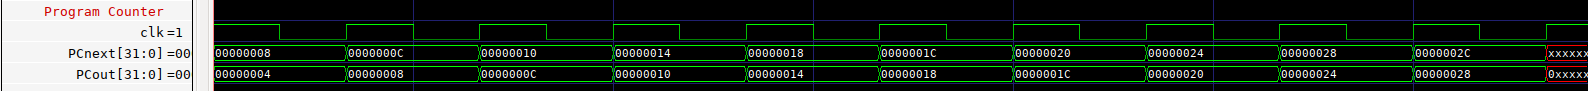
\includegraphics[width=\columnwidth]{Lab-Tex/Lab6-images/p1.png}
    \captionof{figure}{Wave output of program counter}
    \medskip
\endgroup

\subsection{Staggered Output Demonstration}

The waveform below demonstrates the output delay of the \cc{PCnext} signal as a way to show that the pipeline registers function as required. 

\begingroup
    \centering
    \medskip
    %width=\columnwidth
    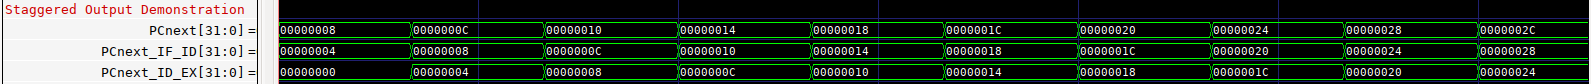
\includegraphics[width=\columnwidth]{Lab-Tex/Lab6-images/o1.png}
    \captionof{figure}{Wave output PCnext at various stages}
    \medskip
\endgroup



\subsection{Pipelining Stage 1}

The outputs of the PC adder and Instruction Memory (IM) are fed as inputs into the first pipeline register.

\begingroup
    \centering
    \medskip
    %width=\columnwidth
    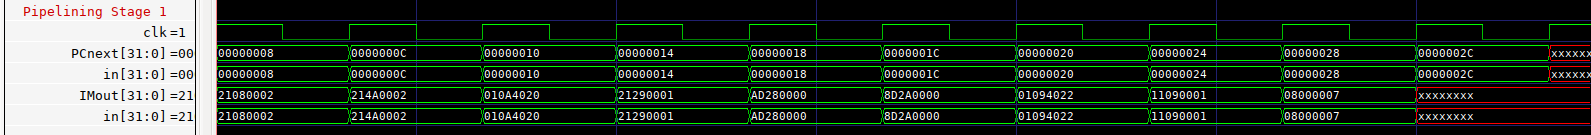
\includegraphics[width=\columnwidth]{Lab-Tex/Lab6-images/p2.png}
    \captionof{figure}{Wave output of stage 1}
    \medskip
\endgroup

\subsection{Pipelining Stage 2}

Comparing PCnext and IMout in the screenshot below to the signals above, we see that there is a stage delay. In the screenshot above, \cc{PCnext} is \cc{0x8} on the first cycle, while \cc{PCnext-IF-ID} is \cc{0x4} in the screenshot below.\\

Aside from the delays, we can also clearly the five stage pipeline begin to play out. In the first cycle, the \cc{readRegisterOne} and \cc{readRegisterTwo} signals are blank, implying the \cc{IF} stage. In the \cc{ID} stage, we see that the CPU now know which registers to fetch data from. However, the \cc{writeRegister} and \cc{writeData} signals only receive their values in the fifth cycle, or the \cc{WB} stage. \\

Interestingly, \cc{writeEnable} is activated earlier, However, this is a side effect of the fact the first instruction in the IM is \cc{0x00000000}, which triggers an R-type control behavior. Nevertheless, this does not affect the program as only \cc{0} is written into the \cc{\$zero} register. We also see the \cc{writeEnable} signal deactivate in the 9th stage, which is the \cc{WB} stage for the \cc{sw} instruction. \\

\begingroup
    \centering
    \medskip
    %width=\columnwidth
    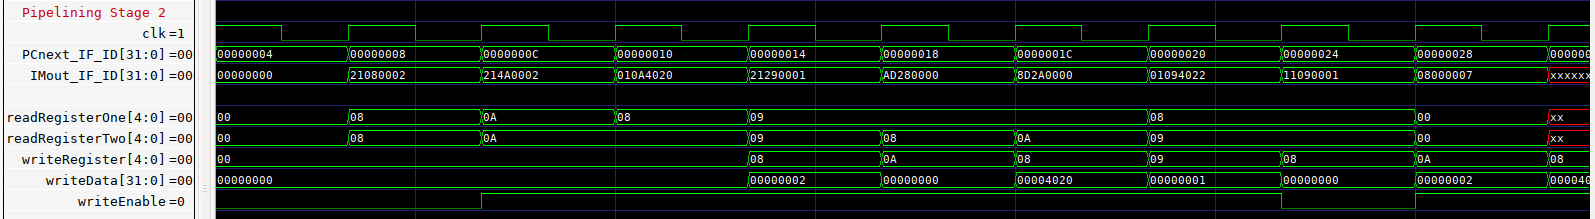
\includegraphics[width=\columnwidth]{Lab-Tex/Lab6-images/p3.png}
    \captionof{figure}{Wave output of stage 2}
    \medskip
\endgroup

\subsection{Pipelining Stage 3}

The \cc{PCnext-ID-EX} signal helps keep track of the instruction at which the behavior is occurring. \\

The first block shows that the ALU takes in the output of the register file directly. While the second block demonstrates that there is a mux selection between the register output and the sign-extended output for the ALU's second input. \\

There is also a mux-selection that occurs for the write register, which was moved to stage 3 for this implementation. \\

The muxes select appropriately according to the control signals from the pipeline register. For example, we see that \cc{ALUin2} selects the register file output for the first two instructions (which are I-type), then selects the sign-extended output for the third instruction (R-type). \\

As a result, register \cc{\$t0} and \cc{\$t2} end up with value 2 in their respective \cc{WB} stages. \textbf{However, the third instruction is supposed to update the value of register \cc{\$t0} to 4. In this implementation, because there is no data forwarding, nor is there a stall, register \cc{\$t0} is updated to value 0. This is the result of a data hazard, which is unsupported in this pipeline.}\\

\begingroup
    \centering
    \medskip
    %width=\columnwidth
    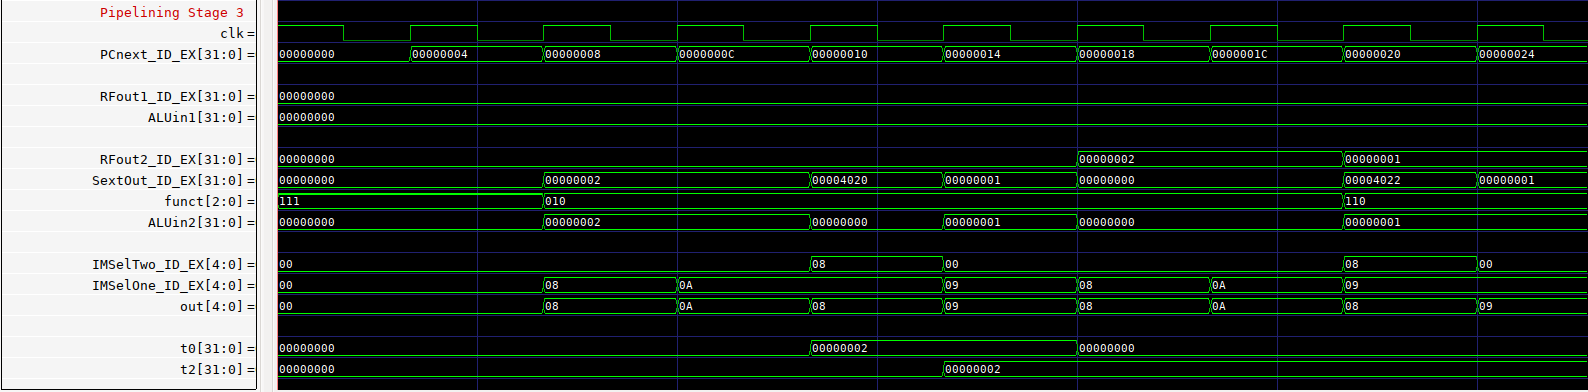
\includegraphics[width=\columnwidth]{Lab-Tex/Lab6-images/p4.png}
    \captionof{figure}{Wave output of stage 3}
    \medskip
\endgroup


\subsection{Pipelining Stage 4}

In this stage, we are able to better see the reason why register \cc{\$t0} gets incorrectly updated. The \cc{RFWriteReg-EX-MEM} signal carries register \cc{\$t0} at cycle 6. At this point, the \cc{RFout2-EX-MEM} signal should be carrying the value 4; however, since register \cc{\$t2} write back hasn't been completed, this is not the case. The failure to update results in a cascading set of problems, where branching would be doomed because the value will never reach 1, which is the branch condition! The \cc{BranchCtrl} signal shows that the instruction is a branch instruction, while the \cc{Branch} signal shows whether this branch is obeyed or not. Since it is not obeyed, we see that the instructions linearly carry through to the next instruction. \\

\begingroup
    \centering
    \medskip
    %width=\columnwidth
    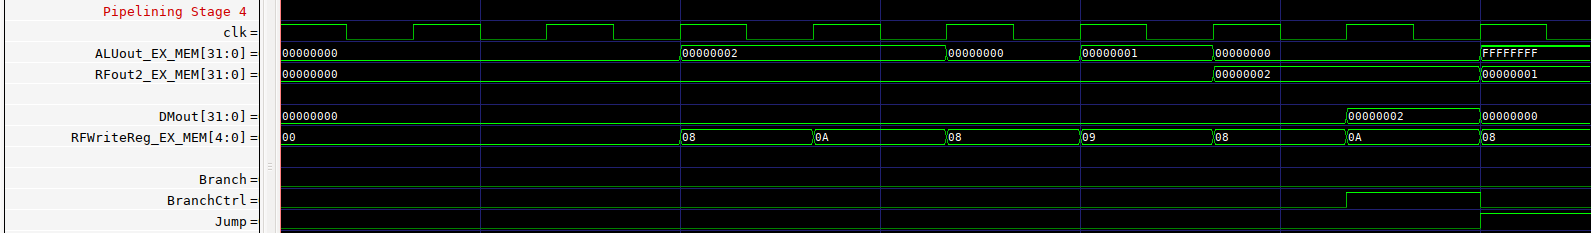
\includegraphics[width=\columnwidth]{Lab-Tex/Lab6-images/p5.png}
    \captionof{figure}{Wave output of stage 4}
    \medskip
\endgroup

\subsubsection{Introducing Jump}

The provided diagram only allows support for branch instructions. Hence, the wiring was adjusted to allow for jumping. Originally, the \cc{PCbranch-EX-MEM} signal and the \cc{PCnext} signal is fed into a mux which decides the \cc{PCin}. \\

To allow for jumps, the the \cc{PCbranch-EX-MEM} signal and the \cc{jumpAddress} signals are fed into a mux. The output of this mux is then fed into another mux along with \cc{PCnext}, the output of which is fed into \cc{PCin}. Thus, to support jump instructions, the implementation requires another mux. \\

The first mux selects for jump or branch addresses using the signal \cc{Branch}. However, for the second mux, in this implementation, a new signal had to be created called PCSrc, which was an OR beteween \cc{jump} and \cc{branch}. This is because the \cc{PCnext} signal must select for the signal that is \textit{not} \cc{PC + 4} if either jump or branch are enabled. \\

\begingroup
    \centering
    \medskip
    %width=\columnwidth
    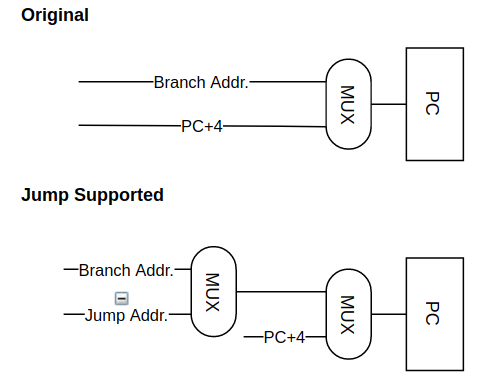
\includegraphics[width=0.65\columnwidth]{Lab-Tex/Lab6-images/p6.png}
    \captionof{figure}{Diagram depicting jump instruction}
    \medskip
\endgroup
\\
Looking back at the signals, we see that the jump signal is enabled at the correct time. In our instructions, the jump instruction is responsible for carrying the loop back to a previous label. \\

The signals show that the jump instruction is selecting the correct address to jump to, but the program stops working shortly after. The \cc{sub} instruction is correctly selected from the IM, confirming the jump instruction is actually carried out. 
\\

\begingroup
    \centering
    \medskip
    %width=\columnwidth
    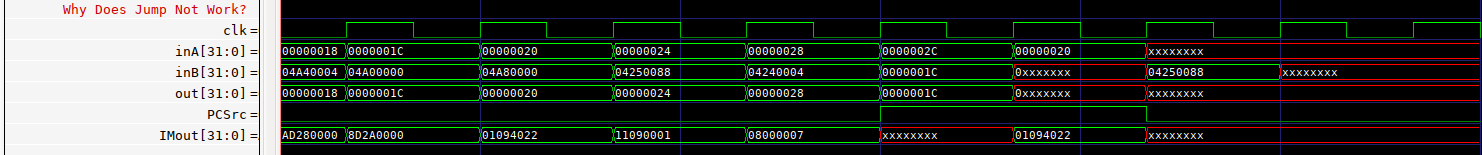
\includegraphics[width=\columnwidth]{Lab-Tex/Lab6-images/p7.png}
    \captionof{figure}{Diagram depicting why jump works}
    \medskip
\endgroup

The data hazard which led to register \cc{\$t0} storing a value of 0, continues to cause a problem. The \cc{sub} instruction now results in register \cc{\$t0} storing -1. \\

\textbf{However, the root of the problem lies in the mux selecting a corrupted value for the next address, which in turn corrupts the output of the second mux as well, because it is set to the \cc{beq} instruction!} The screenshot below shows the inputs and output of the first mux selecting between the branch address and jump address. We see that in the 7th cycle, there is a corrupt output, which occurs because there is a gap in instruction selection. \\

The gap in instructions can be seen by the undefined \cc{opcode} signal in between the defined \cc{opcode} signals towards the end. \textbf{The gap occurs because the pipeline naturally takes in the instruction after the jump, while the jump is still being "computed". As a result of taking in a non-existent instruction, there are corruptions in signals. This could be best fixed by a stall after the jump to prevent taking in nonsense instructions. }\\

\begingroup
    \centering
    \medskip
    %width=\columnwidth
    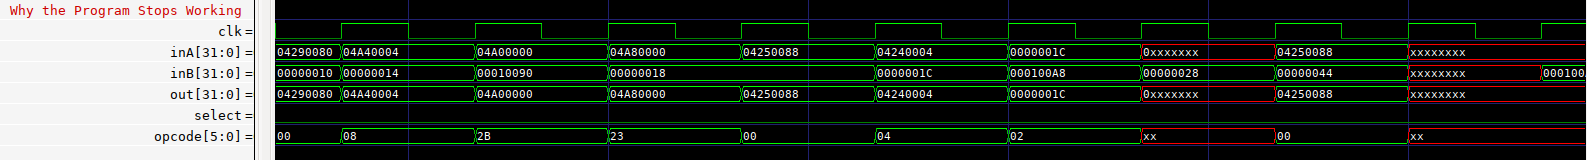
\includegraphics[width=\columnwidth]{Lab-Tex/Lab6-images/p8.png}
    \captionof{figure}{Diagram depicting why the program fails after jump}
    \medskip
\endgroup


\section{Conclusion}

The two reasons why the program failed to run were the data hazard which ensured that register \cc{\$t0} would never have the correct output and the corrupt address selection because of naturally in-taking a non-existent instruction into the pipeline.


%%%%%%%%%%%%%%%%%%%%%%%%%%5
% BIBLIOGRAFIA 
% Estilo de bibliografia ABNT. Se não tiver instalado, mude para plain ou ieeetr

%\bibliographystyle{plain} % Inclua isso se não tiver ABNTEX instalado
% \begin{thebibliography}{refs}
% \bibitem{}
\printbibliography
% \end{thebibliography}
\end{document}